\section{System Model and Control Objective}\label{sec:model}
\begin{figure}[t]
\centering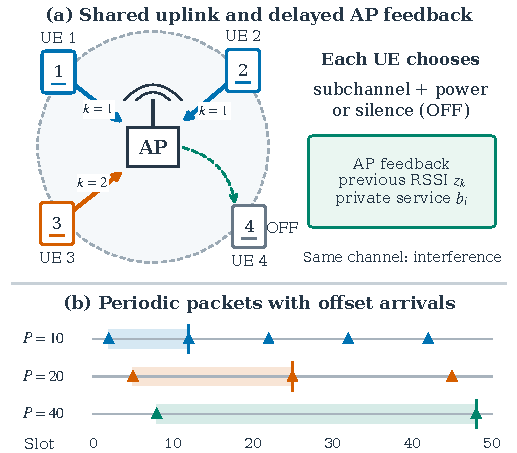
\includegraphics[width=\columnwidth]{figures/system_scenario.pdf}
\caption{Periodic uplink access. Solid arrows illustrate transmissions;
UEs 1 and 2 reuse a subchannel and interfere at the AP. Dashed feedback is
received even during silence. Shading marks the first packet window in each
illustrative traffic class; triangles denote arrivals and vertical bars its
deadline. Physical slots are synchronized, while arrival phases differ.}
\label{fig:scenario}
\end{figure}
\subsection{Periodic uplink and accumulated service}
Figure~\ref{fig:scenario} illustrates an access point (AP) receiving uplink
packets from $N$ devices over $K$
orthogonal subchannels. Slots have duration $\tau$, and each subchannel has
bandwidth $B$. Device $i$ generates a packet of $L_i$ bits at
$a_{i,m}=\varphi_i+mP_i$, with deadline $d_{i,m}=a_{i,m}+P_i$.
The phase $\varphi_i$ is drawn independently and uniformly from
$\{0,\ldots,P_i-1\}$. Physical slots are synchronized; asynchronous traffic
refers to the packet-arrival phases. At most one packet is pending per device.

In slot $t$, device $i$ selects $a_i(t)\in\{\OFF\}\cup
(\{1,\ldots,K\}\times\mathcal P)$, where $\mathcal P$ is the positive
discrete-power menu. Let $k_i(t)$ and $p_i(t)$ denote its chosen subchannel and
power, with $p_i(t)=0$ for $\OFF$. The noise power per subchannel is $\sigma^2$.
The AP decodes each device's signal by treating interference as noise.
For an active device,
\begin{align}
\gamma_i(t)&=\frac{p_i(t)g_i}
 {\sigma^2+\sum_{j\ne i:k_j(t)=k_i(t)}p_j(t)g_j},\label{eq:sinr}\\
b_i(t)&=\tau B\log_2(1+\gamma_i(t)),\qquad e_i(t)=\tau p_i(t).
\label{eq:service}
\end{align}
The gain $g_i$ is static and identical across subchannels within an instance;
subchannel selection controls co-channel interference.
For silence, $b_i(t)=e_i(t)=0$.

We use an ideal accumulated-mutual-information model, motivated by incremental
redundancy hybrid ARQ~\cite{caire2001}. A packet completes once the sum of its
slot services reaches $L_i$. Even if its final transmission
provides excess service, a device occupies and pays for the whole slot. At each
slot boundary, the environment first applies service, then settles expiring
packets, and finally releases new packets. Unfinished bits are discarded at
expiry. A device without a pending packet must select $\OFF$ but continues
receiving observations. We measure radiated transmit energy using
\eqref{eq:service}.

\subsection{Causal execution information}
At a slot's start, device $i$ knows its remaining bits $s_i(t)$, remaining time
$D_i(t)$, its packet size and period, and its preceding action and outcome.
The AP supplies the previous slot's per-subchannel received power $z_k(t-1)$,
including noise, and the device's private service feedback $b_i(t-1)$.
It supplies no scheduling decision. Devices do not exchange messages, and the
policy receives no device identifier, global slot index, topology, or other
devices' queues, phases, gains, and actions.

These observations contain useful channel information. After transmitting at
power $p$ on subchannel $k$, a device can infer
\begin{equation}
\widehat\gamma=2^{b/(\tau B)}-1,\qquad
\widehat I=\frac{z_k}{1+\widehat\gamma},\qquad
\widehat g_i=\frac{z_k-\widehat I}{p}.\label{eq:estimate}
\end{equation}
The gain estimate is retained across packets. Exact feedback and a static
channel make this estimate exact after a transmission in the ideal model;
the remaining uncertainty includes other devices' future actions. All
distributed baselines use the same permitted observation stream.

\subsection{Energy and per-device reliability}
Let $c_{i,m}=1$ if packet $m$ of device $i$ expires unfinished. For a fixed
instance, the policy objective is
\begin{align}
\min_{\pi}\quad &J(\pi)=\limsup_{T\to\infty}\frac{1}{NT}
 \E_\pi\!\left[\sum_{t=0}^{T-1}\sum_i e_i(t)\right],\label{eq:objective}\\
\text{s.t.}\quad &\limsup_{M\to\infty}\frac{1}{M}
 \E_\pi\!\left[\sum_{m=0}^{M-1}c_{i,m}\right]\le\epsilon,
 \quad \forall i.\nonumber
\end{align}
The per-device constraints assign the same violation allowance to every
device. We train the policy across random instances using a penalized reward
and each device's local history. Section~\ref{sec:experiments} defines the
finite-episode reliability criterion used for evaluation.
